\documentclass[xetex,aspectratio=43]{beamer}

\usepackage{res/lections}

\preamble

\title{Память и ПЛИС}

\begin{document}

    \titleslide

    \tocslide

\section{Динамическая память}

\begin{frame}{Память: статическая и динамическая}
    \begin{outline}[itemize]
        \1 Статическая --- на триггерах (обычно D). Применяется:
            \2 Где её нужно немного (микроконтроллеры, память настроек и часов и т.д.)
            \2 Где нужна память, не требующая дополнительных расходов времени (регистры, кэш)
        \1 Динамическая --- на схемах с [обычно кратковременной] памятью состояния
            \2 \href{https://en.wikipedia.org/wiki/Magnetic-core_memory}{Ферритовые кольца или сердечники} (могла быть энергонезависимой)
            \2 \href{https://en.wikipedia.org/wiki/Racetrack_memory}{Беговая память} --- на принципе перемещения магнитных доменов в нанотрубках
            \2 Специальные ЭЛТ --- \href{https://en.wikipedia.org/wiki/Williams_tube}{Трубки Ульямса}
            \2 Конденсаторы
    \end{outline}
\end{frame}

\begin{frame}{DRAM: -1 приближение}
    \alert{В минус первом приближении (4-битный процессор, 1 слово в строке)}

    \begin{figure}
        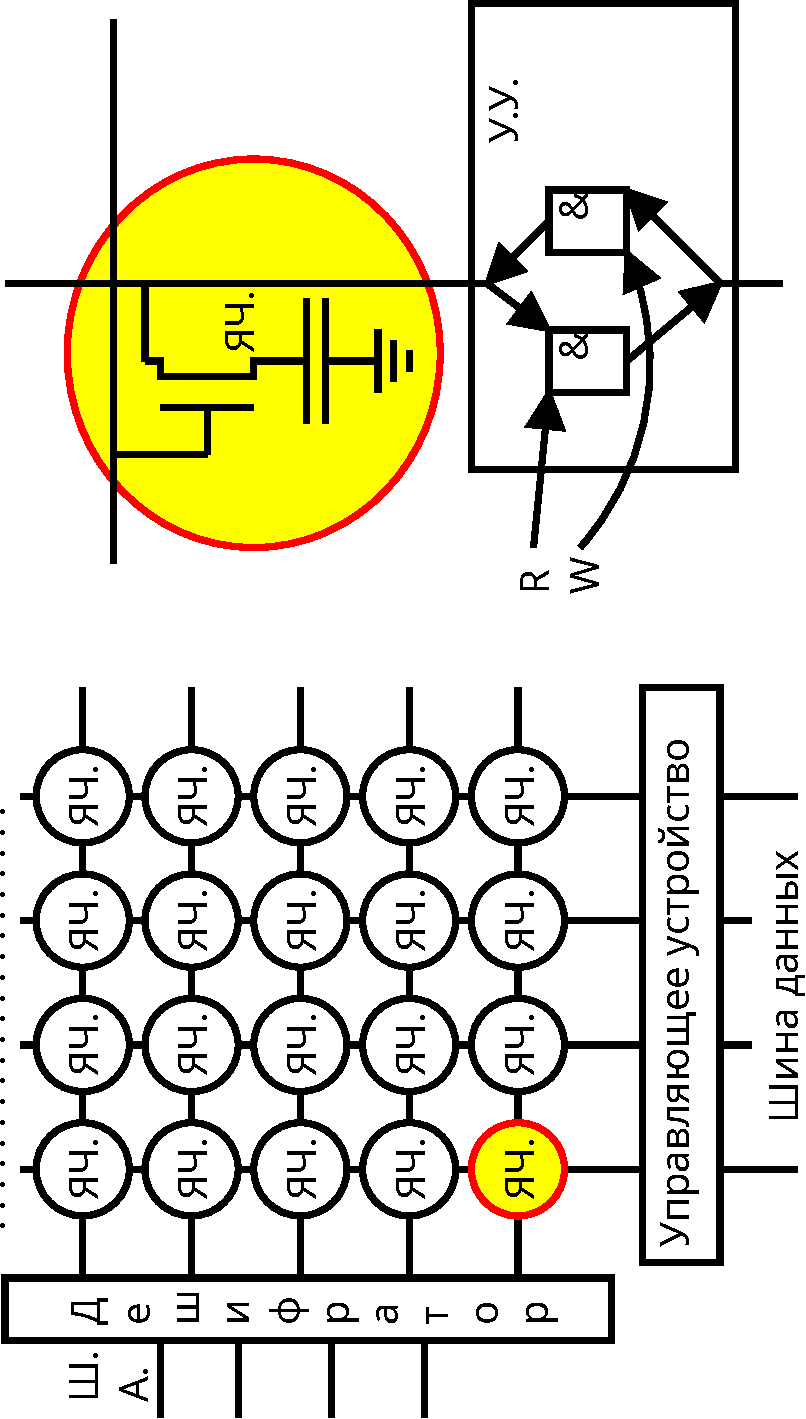
\includegraphics[angle=-90,origin=c,height=0.75\textheight]{img/\jobname/dram-crop.pdf}
        \vspace{-20mm}
    \end{figure}

\end{frame}

\begin{frame}{DRAM: реальность}
    \begin{outline}[itemize]
        \1  \href{https://en.wikipedia.org/wiki/Dynamic_random-access_memory\#History}{Технологически конденсатор выполняется вместе с транзистором} и почти не
        требует дополнительного места: может быть использована ёмкость P-N
        перехода
        \pause
        \1 \href{https://en.wikipedia.org/wiki/Dynamic_random-access_memory\#To_write_to_memory}{По горизонтали --- не шина данных с одним словом, а «широкая» строка}, нужные участки которой управляющая схема мультиплексирует при чтении из памяти и демультиплексирует при записи (а «ненужные» просто перезаписывает)
    \end{outline}
\end{frame}

\begin{frame}{Flash-память: элементная база}
    \begin{itemize}
        \item
        \href{http://en.wikipedia.org/wiki/Floating-gate_transistor}{Транзистор
            с плавающим затвором} Эти полевые транзисторы могут при подаче
        \emph{достаточно} высокого или \emph{достаточно} низкого потенциалов
        (т.е. заметно больше 1 или заметно меньше 0) на управляющий вход
        запоминать своё состояние. После нескольких миллионов срабатываний
        транзистор необратимо портится (поэтому у Flash ограничено количество
        перезаписей). Этим эффектом, так же как и широкой петлёй гистерезиса
        (хотя природа этого совершенно иная), можно пользоваться для хранения
        данных.
        \item
        На основе таких транзисторов делается
        \href{http://en.wikipedia.org/wiki/Flash_memory}{флэш-память}
    \end{itemize}
\end{frame}

\begin{frame}{Flash-память: реализация NAND}
    \begin{figure}
        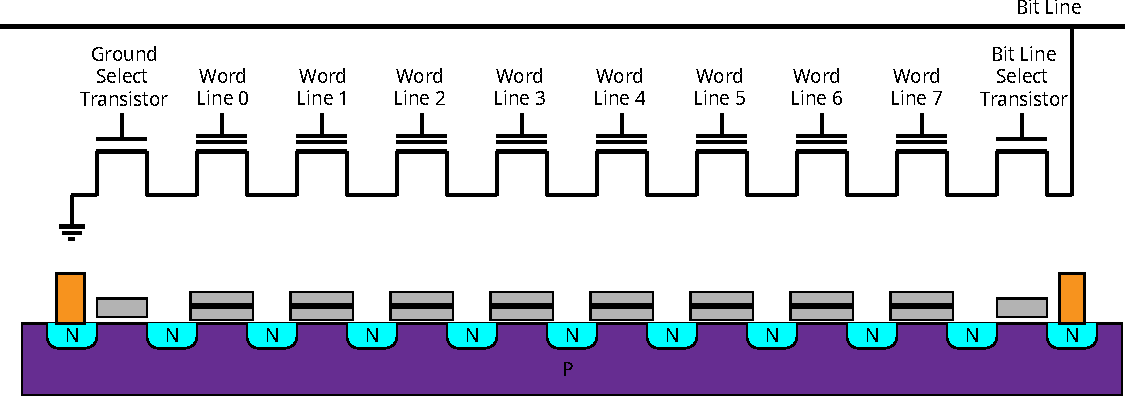
\includegraphics[height=0.25\textheight]{img/\jobname/nand.pdf}
    \end{figure}

    \begin{itemize}
        \tightlist
        \item
        Для чтения на все слова, кроме читаемого, подаётся небольшой
        «приоткрывающий» потенциал. Ток течёт с соответствующих открытым
        транзисторам битовых линий в землю.
        \item
        Для программирования (открытия затвора, установки в бита 0) надо
        небольшим потенциалом «приоткрыть» все линии слов и подать сильный
        сигнал на пересечения нужных слова и бита.
    \end{itemize}
\end{frame}

\begin{frame}[fragile]{Flash-память: особенности NAND, альтернативы}
    \begin{itemize}
        \tightlist
        \item
        Из-за особенностей изготовления транзисторов, сброс (в 1) по словам
        или ещё большим блокам
        \item
        Для SSD введена операция
        \href{https://ru.wikipedia.org/wiki/TRIM}{\texttt{TRIM}}, которая
        говорит накопителю, что блок памяти свободен и может использоваться
        для оптимизации с целью увеличения ресурса перезаписи

        \pause

        \item
        Альтернативная технология ---
        \href{https://en.wikipedia.org/wiki/Phase-change_memory\#Challenges}{память
            на основе изменений фазового состояния халькогенидов} --- обладает
        потенциально лучшими характеристиками, уже используется коммерчески
        (Например, кэш для ФС Intel Optane™), но тоже со временем деградирует
    \end{itemize}

\end{frame}

\section{ПЛИС}

\begin{frame}{Что это и зачем?}
        Что это?

        \begin{itemize}
            \tightlist
            \item
            \defn{Программируемые логические интегральные схемы (Programmable Logic Device)}{ интегральные схемы,
            физический уровень которых (реализующий логику) можно задавать
            программно}

            \begin{itemize}
                \tightlist
                \item
                программируются связи между компонентами схемы
            \end{itemize}
        \end{itemize}

        Зачем?

        \begin{itemize}
            \tightlist
            \item
            Применяются для эффективной реализации (быстродействие --- заметно
            медленнее серийных микросхем, существенно быстрее микропрограмм,
            принципиально быстрее обычной программной реализации) специфических
            задач

            \begin{itemize}
                \tightlist
                \item
                прототипирование, единичное или мелкосерийное производство
                \item
                микропроцессоры встроенных ЭВМ
            \end{itemize}
        \end{itemize}
\end{frame}

\begin{frame}{Какие бывают ПЛИС?}
        \begin{itemize}
            \tightlist
            \item
            Простые ПЛИС --- логические функции, в т.ч. довольно сложная логика,
            но явно задаются через вентили «и», «или», «не»
            \item
            CPLD (Complex Programmable Logic Device) --- несколько более
            высокоуровневые, содержат внутренние шины, более сложные элементы
            \item
            Программируемая пользователем вентильная матрица (Field-Programmable
            Gate Array, FPGA) --- содержит готовые регистры, компоненты АЛУ и т.д.
        \end{itemize}
\end{frame}

\begin{frame}{Пример: ПЛИС типа GAL (Gateway Array Logic)}
    \begin{figure}
        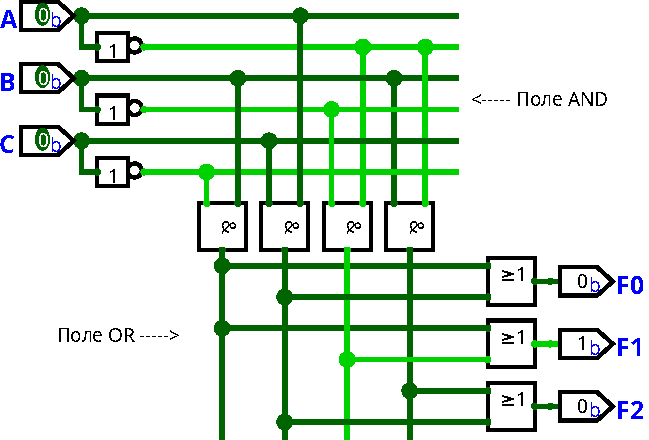
\includegraphics[height=0.5\textheight]{img/\jobname/PLD.pdf}
    \end{figure}
    Схема на примере вычисляет функции, представленные в ДНФ:

    \begin{eqnarray*}
    F_0 = B \wedge\neg C \vee A\wedge C\ \\
    F_1 = B \wedge\neg C \vee \neg A \wedge \neg B \\
    F_2 = A\wedge C \vee \neg A \wedge B
    \end{eqnarray*}
\end{frame}

\begin{frame}{Пример: ПЛИС типа GAL (замечания)}
    \begin{outline}[itemize]
        \1 Входов у вентилей обычно больше, чем 2
        \1 Как реализуются перемычки в полях OR и AND?

        \2 «пережиганием» (одноразовое программирование); мультиплексором с управлением статической памятью; транзистором с плавающим затвором
    \end{outline}
\end{frame}

\begin{frame}{Как программировать ПЛИС и чего можно добиться?}
        \begin{itemize}
            \tightlist
            \item
            Специальные языки, например Verilog Hardware Definition Language
            \item
            САПР (даже Logism)

            \begin{itemize}
                \tightlist
                \item
                Т.е. почти всё, что есть (было и будет) в данном курсе, можно
                сделать на ПЛИС
            \end{itemize}
            \item
            \textbf{Hardware-Software CoDesign} --- подход, подразумевающий
            совместную разработку специализированных ПО и оборудования

            \begin{itemize}
                \tightlist
                \item
                На кафедре системного программирования СПбГУ --- Булычев, Медведев,
                Терехов: https://scholar.google.com/scholar?q=HasCOL+SPbU
            \end{itemize}
        \end{itemize}
\end{frame}

\section*{}

 \begin{frame}{Вопросы}
    \begin{itemize}
        \item
        Как организована динамическая память?
        \item
        Как организована NAND-память?
        \item
        Что такое ПЛИС? Зачем они нужны и какие бывают?
        \item
        Опишите структуру ПЛИС типа GAL с полями AND и OR
        \item
        Как программируются ПЛИС?
    \end{itemize}
\end{frame}

\postamble

\end{document}
